%%%%%%%%%%%%%%%%%%%%%%%%%%%%%%%%%%%%%%%%%
% University/School Laboratory Report
% LaTeX Template
% Version 3.1 (25/3/14)
%
% This template has been downloaded from:
% http://www.LaTeXTemplates.com
%
% Original author:
% Linux and Unix Users Group at Virginia Tech Wiki 
% (https://vtluug.org/wiki/Example_LaTeX_chem_lab_report)
%
% License:
% CC BY-NC-SA 3.0 (http://creativecommons.org/licenses/by-nc-sa/3.0/)
%
%%%%%%%%%%%%%%%%%%%%%%%%%%%%%%%%%%%%%%%%%

%----------------------------------------------------------------------------------------
%	PACKAGES AND DOCUMENT CONFIGURATIONS
%----------------------------------------------------------------------------------------

\documentclass{article}

\usepackage[version=3]{mhchem} % Package for chemical equation typesetting
\usepackage{siunitx} % Provides the \SI{}{} and \si{} command for typesetting SI units
\usepackage{graphicx} % Required for the inclusion of images
\usepackage{natbib} % Required to change bibliography style to APA
\usepackage{amsmath} % Required for some math elements 
\usepackage{hyperref}
\usepackage[a4paper,margin=0.5in]{geometry}
\setlength\parindent{0pt} % Removes all indentation from paragraphs

\renewcommand{\labelenumi}{\alph{enumi}.} % Make numbering in the enumerate environment by letter rather than number (e.g. section 6)

%\usepackage{times} % Uncomment to use the Times New Roman font

%----------------------------------------------------------------------------------------
%	DOCUMENT INFORMATION
%----------------------------------------------------------------------------------------

\title{Gate Detection} % Title

\author{Philipp \textsc{Duernay}} % Author name

\date{\today} % Date for the report

\begin{document}
\maketitle
% If you wish to include an abstract, uncomment the lines below
% \begin{abstract}
% Abstract text
% \end{abstract}

%----------------------------------------------------------------------------------------
%	SECTION 1
%----------------------------------------------------------------------------------------

\section{Recap}
In the last meeting from 02.02.2018 several next steps were defined:
\begin{enumerate}
	\item \textbf{Get Real(er) Data.}
	\item \textbf{Investigate reason for bias in the upper left corner.}
	\item \textbf{New data with thicker gates.}
	\item \textbf{Visualize Confidence for each prediction/distance}
	\item \textbf{Implement SSD}
	\item \textbf{Reading.}
	\item (\textbf{Visualize what model has learned.})
\end{enumerate}

\section{Data}

\subsection{Synthetic Dataset}
So far only the gates of IROS 2017 were used which have a very thin frame and are hard to detect. Also the placement of the gates was very random and did not fit to the natural properties of the image. One could have a top view of a gate on the background of sky for example. To generate a setting which resembles more what the drone will see the new dataset only contains camera poses with slight changes in roll and pitch angle. The view on gates is from the front or side. Also the gates from IROS 2016 are included which contain thicker frames. Examples can be seen in \autoref{fig:data}.

\begin{figure}[h]
	\centering
	\begin{minipage}{0.24\textwidth}
		\centering
		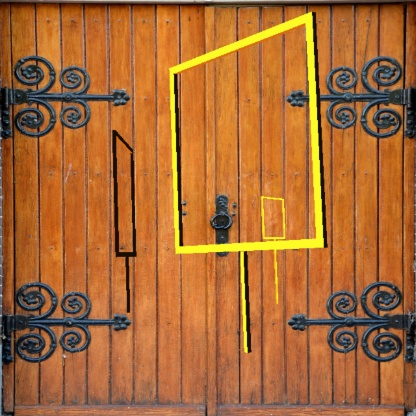
\includegraphics[width=\textwidth]{fig/sample}
		
	
	\end{minipage}
	%\hspace{3cm}
	\begin{minipage}{0.24\textwidth}
		\centering
		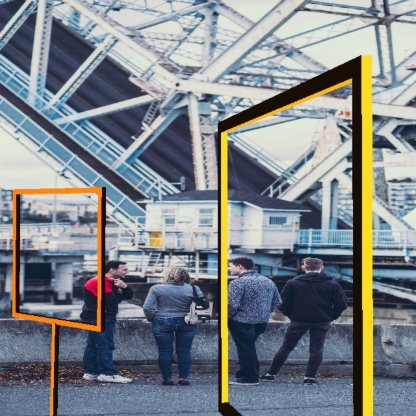
\includegraphics[width=\textwidth]{fig/sample2}
	\end{minipage}
	\begin{minipage}{0.24\textwidth}
		\centering
		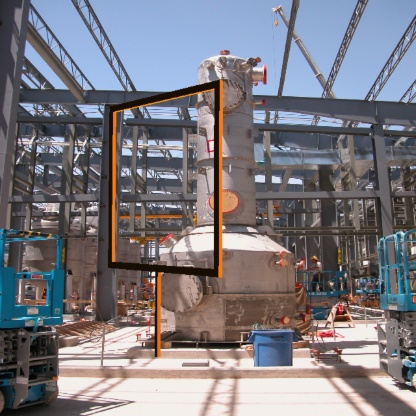
\includegraphics[width=\textwidth]{fig/sample3}
	\end{minipage}
	\begin{minipage}{0.24\textwidth}
		\centering
		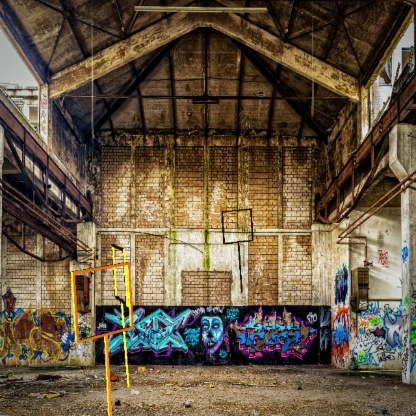
\includegraphics[width=\textwidth]{fig/sample4}
	\end{minipage}
	\caption{Images with the new gate, less random positions. All displayed images contain one or more gates.}
	\label{fig:data}
\end{figure}

\subsection{Real Data}
A dataset with 500 gates was labeled by Shuo and can be used for testing/training \autoref{fig:gates}. The models trained on synthetic data were tested on the set but no gates were detected.
\begin{figure}[h]
	\centering
	\begin{minipage}{0.4\textwidth}
		\centering
		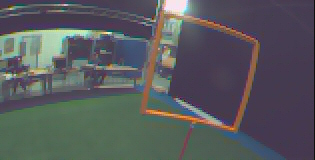
\includegraphics[width=\textwidth]{fig/sample_real}
	\end{minipage}
	%\hspace{3cm}
	\begin{minipage}{0.4\textwidth}
		\centering
		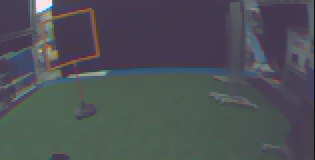
\includegraphics[width=\textwidth]{fig/sample_real1}
	\end{minipage}
	\caption{A dataset with 500 gates was labeled by Shuo and can be used for testing/training.}
	\label{fig:gates}
	\end{figure}
\section{Method}

\subsection{Yolo}

Two parts of the Yolo-Object-Detector were investigated further.

\subsubsection{Bias upper left corner}

In the last videos we saw that the model tend to predict a box in the upper left corner. This could have been due to a bias in the dataset or a bias in the model. If we look at a heatmap of the label distribution of the training set there wasn't a peak at the upper left corner that would indicate such a bias. Also yolo should only output a box if it detects an object in a certain area, there should be no bias by design. The behavior was due to a stupid mistake, while training the model in yuv-color space the test samples were fed in rgb-space. After converting the images properly the "bias" was gone. For the fact that the prediction was in the wrong color space the results were still surprisingly good.

\subsubsection{Image Augmentation}

As mentioned in the last report, Yolo relies heavily on image augmentation to avoid overfitting and to artificially increase the training set. This contains random cropping of the image, translating and color changing. However, the orange color is one of the main distinctive features of the gates we want to detect. Therefore image augmentation was deactivated for now to see the effect on performance.

\subsection{SSD}

SSD is another fast deep-learning based object detector and would be nice to compare against Yolo. The implementation is theoretically working, practically the training does not converge yet :(. That's why unfortunately no results are available yet.

\subsection{Other Methods}

Some literature study was done on alternative methods. Findings can be found in the appendix.

\section{Evaluation}

\subsection{Experiment I}

In this experiment the models were tested on a set of 1000 images on random backgrounds. Similar to "Bounding Box Detection" in the last report \autoref{fig:bb}. The big and the small version of yolo are tested. Each model with different amount of training samples.

\begin{figure}[h]
	\centering
	\begin{minipage}{0.45\textwidth}
		\centering
	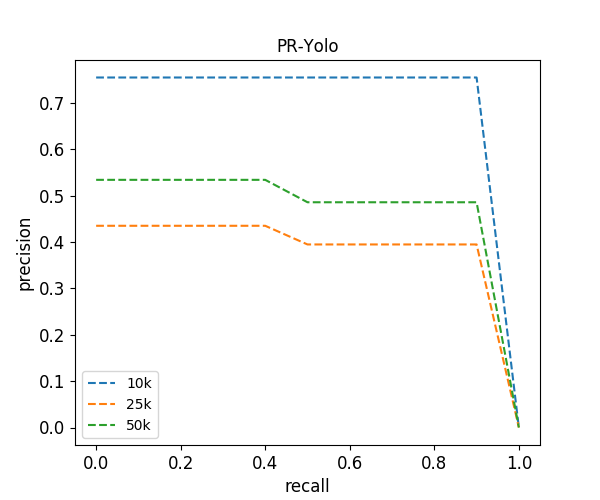
\includegraphics[width=\textwidth]{fig/pr_yolo}
	\end{minipage}
	%\hspace{3cm}
	\begin{minipage}{0.45\textwidth}
		\centering
	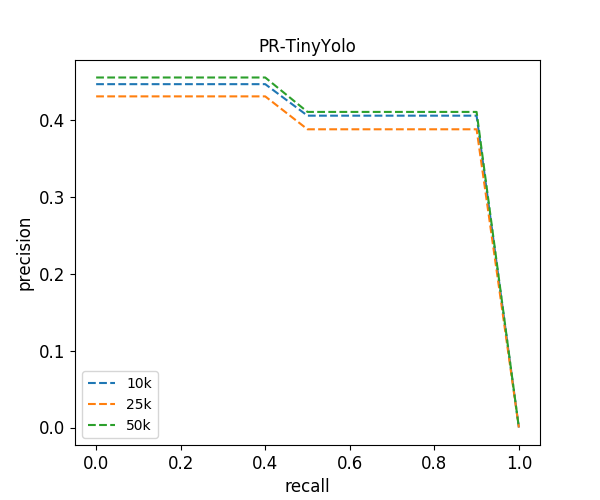
\includegraphics[width=\textwidth]{fig/pr_tinyyolo}
	\end{minipage}
	\caption{The plot shows the average precision-recall plot across all images.}
	\label{fig:bb}
\end{figure}

\subsection{Experiment II}

This experiment is similar to lasts report "Single Gate Detection". \autoref{fig:stream_yolo} shows the performance of the big yolo, \autoref{fig:stream_tinyyolo} shows the performance of the small yolo version. The plots show the localization error (L1 distance of the bounding box coordinates) in blue and the classifier confidence in percent in orange. The corresponding videos are at \url{https://www.youtube.com/watch?v=FEtm27U0tlQ} for the big one and \url{https://www.youtube.com/watch?v=Bzs5ZpMdpL8} for the small one.
\begin{figure}[hbtp]
	\centering
	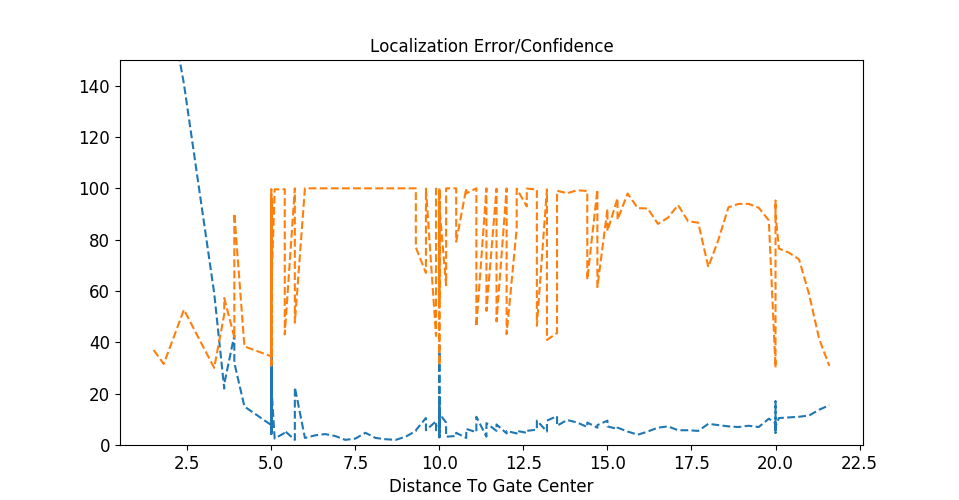
\includegraphics[width=0.9\textwidth]{fig/stream3_yolo}
	\label{fig:stream_yolo}
\end{figure}

\begin{figure}[hbtp]
	\centering
	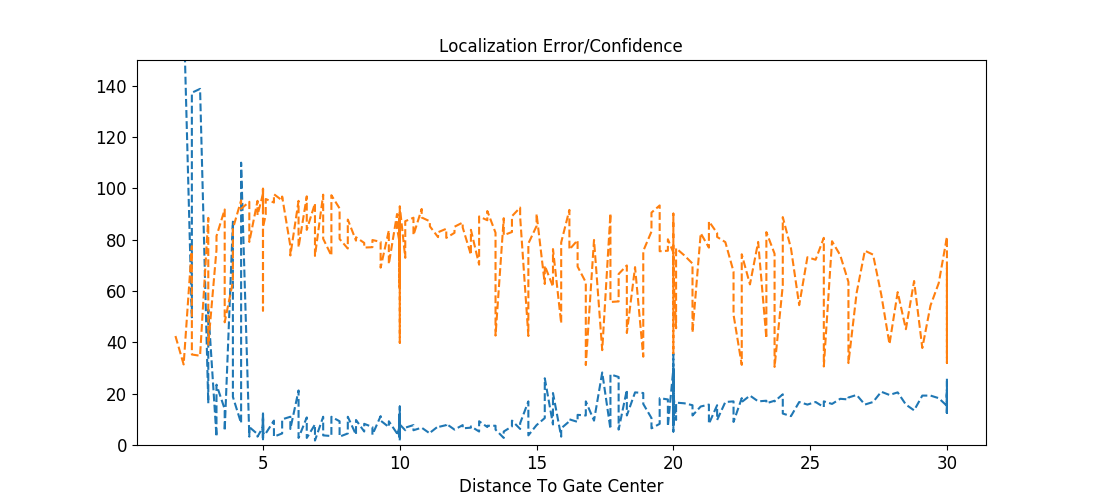
\includegraphics[width=0.9\textwidth]{fig/stream3_tinyyolo}
	\label{fig:stream_tinyyolo}
\end{figure}

\subsection{Speed}

Some speed performance tests were done by evaluating 60 images in 6 batches:

\begin{table}[htbp]
	\centering
	\caption{}
	\begin{tabular}{|l|l|l|}
		\hline
		Frames Per Second & Yolo & TinyYolo \\ \hline
		i5 CPU & 0.43 $\pm$ 0.03 & 1.6 $\pm$ 0.1 \\ \hline
		Titan GPU & 7.33 $\pm$ 2.51 & 5.9 $\pm$ 1.2 \\ \hline
	\end{tabular}
	\label{}
\end{table}


\section{Thoughts \& Conclusions}


\begin{enumerate}
	\item \textbf{Performance} After removing the image augmentation and on the new dataset the results improved quite a bit. Especially the amount of false positives decreased. Even a smaller network like tiny yolo could detect some gates As long as there are no differently colored gates on the track we should probably use it as a feature.
	
	\item \textbf{Training Data} Using less training data had minor effects or even improved the results. Which is surprising but means we have to label less data.
	
	\item \textbf{One Stage Detection Framework.} With the current implementation () we have a flexible framework for object detection. A lot of current methods use variants use approaches within this framework. We can work with different base networks, predictor layers, loss functions and training procedures. In a next step we can investigate which architecture is most suitable for our application, based on the available hardware and experiments on real data.
	
	\item \textbf{Speed.} The speed performance results are way below on what the authors state in the papers (Also competing authors), even when running it on a big GPU.

\end{enumerate}

\section{Next Steps}
\begin{enumerate}
		\item \textbf{Read on transfer learning between synthetic and real data}
		\item \textbf{Label real data, start with ~5000 images}
		\item \textbf{Try to simulate 180 degree effect on synthetic images}
		\item \textbf{Investigate how such high speed performance was implemented.}
		\item \textbf{Finally finish SSD}
\end{enumerate}
\newpage
\subsection{Other Methods}

\subsubsection{Traditional Methods}

Usually features are handcrafted or separately learned. The response is fed into a classifier that examines the image in sliding window fashion. Examples are Viola and Jones, Histogram of Gradients and Deformable Part Models \cite{Felzenszwalb,Forsyth,Viola2004}.

The methods are usually pretty fast but not so accurate.

\subsubsection{Two Stage Detectors}

Methods consist usually of two stages.An example is R-CNN\cite{Ren}. 
\begin{itemize}
	\item Object Proposal: A convolutional net proposes regions that contain an object. This is either done in sliding window fashion or in one pass.
	\item Classification: All proposed regions are fed into a classifier. This can either be a "traditional" one or another CNN.
\end{itemize}
These methods are usually pretty accurate but also slow.
\subsubsection{One Stage Detectors}

\begin{figure}[h]
	\centering
	\begin{minipage}{0.4\textwidth}
		\centering
		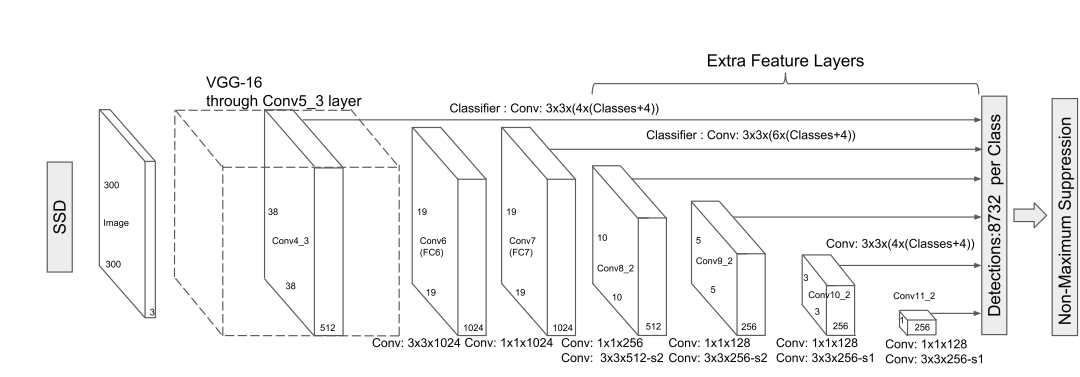
\includegraphics[height=2.5cm]{fig/architecture}
		\caption{Typical Architecture for One Stage Detectors}
		\label{fig:architecture}
	\end{minipage}
	\hspace{2cm}
	\begin{minipage}{0.4\textwidth}
		\centering
		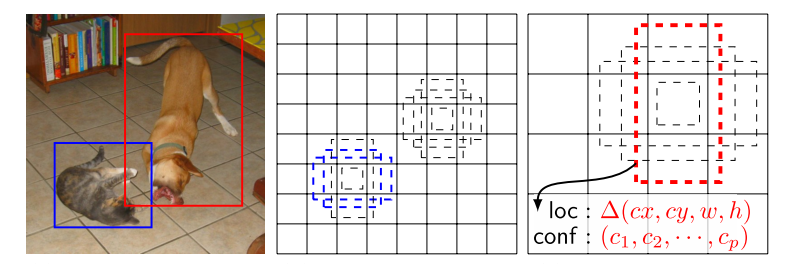
\includegraphics[height=2.5cm]{fig/anchors}
		\caption{Example of \cite{Liu}, the GT box of the cat is matched to two anchor boxes which get responsible for predicting that box. The GT box of the dog is matched to one anchor box.}
		\label{fig:anchors}
	\end{minipage}
\end{figure}

Most current methods rely on the same principle as Yolo/SSD: A convolutional regression layer is stacked on top of a "base network" that has been trained for image classification e.g. VGG-16. The output layer evaluates feature map(s) of the base network and predicts class confidences, and coordinate offsets for a predetermined set of bounding boxes (so called "prior boxes", "anchor boxes" or "default boxes"). The predictions are filtered in a final non-max-suppression step. During training one has to determine which anchor box is responsible for predicting a certain object. This "matching strategy" differs from method to method but is usually based on the intersection-over-union between the ground truth box and anchor box. \autoref{fig:anchors} illustrates the concept. The final loss function calculates the difference between the responsible boxes and the ground truth. Within this framework several approaches exist that either change the base network, modify layers in between and/or tune it to a particular dataset \cite{ChengchengNing2017,Wu,Xiang,Linb,TripathiSanDiego,YoungwanLee}.

A common problem of one stage detectors is the imbalance between background and object samples. Most methods upweigh the positive samples and/or use hard negative mining. \cite{Lin} introduces the \textit{Focal Loss} which focuses on sparse positive samples by design.

%----------------------------------------------------------------------------------------


%----------------------------------------------------------------------------------------
%	BIBLIOGRAPHY
%----------------------------------------------------------------------------------------

\bibliographystyle{abbrv}

\bibliography{literature}

%----------------------------------------------------------------------------------------


\end{document}